\subsubsection{Using reconstructed surface velocities by GPlates}
\label{sec:cookbooks-gplates}
\textit{This section was contributed by Ren{\'e} Ga{\ss}m{\"o}ller}

In a number of model setups one may want to include a surface velocity boundary
condition that prescribes the velocity according to a specific geologic
reconstruction. The purpose of this kind of models is often to test a proposed
geologic model and compare characteristic convection results to present-day
observables in order to gain information about the initially assumed geologic
input. In this cookbook we present \aspect{}'s interface to the  widely used
plate reconstruction software GPlates, and the steps to go from a geologic plate
reconstruction to a geodynamic model incorporating these velocities as boundary
condition.

\paragraph{Acquiring a plate reconstruction.}

The plate reconstruction that is used in this cookbook is included in
the \texttt{data/boundary-velocity/gplates/} directory of
your \aspect{} installation.
For a new model setup however, a user eventually needs to create her own data
files, and so we will briefly discuss the process of acquiring a usable plate
reconstruction and transferring it into a format usable by \aspect{}.
Both the necessary software and data are provided by the GPlates project.
GPlates is an open-source software for interactive visualization of plate
tectonics. It is developed by the EarthByte Project in the School of Geosciences
at the University of Sydney, the Division of Geological and Planetary Sciences
(GPS) at CalTech and the Center for Geodynamics at the Norwegian Geological
Survey (NGU). For extensive documentation and support we refer to the GPlates
website (\url{http://www.gplates.org}). Apart from the software one needs the
actual plate reconstruction that consists of closed polygons covering the
complete model domain. For our case we will use the data provided by
\cite{GTZDSMBSMB12} that is available from the GPlates website under ``Download
$\rightarrow$ Download GPlates-compatible data $\rightarrow$ Global
reconstructions with continuously closing plates from 140 Ma to the present''.
The data is provided under a Creative Commons Attribution 3.0 Unported License
(\url{http://creativecommons.org/licenses/by/3.0/}).

\paragraph{Converting GPlates data to \aspect{} input.}

After loading the data
files into GPlates (*.gpml for plate polygons, *.rot for plate rotations over
time) the user needs to convert the GPlates data to velocity
information usable in \aspect{}. The purpose of this step is to convert from the
description GPlates uses internally (namely a representation of plates as
polygons that rotate with a particular velocity around a pole) to one that can
be used by \aspect{} (which needs velocity vectors defined at individual points
at the surface).

With loaded plate polygon and rotation information the conversion from GPlates
data to \aspect{}-readable velocity files is rather straightforward. First the
user needs to generate (or import) so-called ``velocity domain points'', which
are discrete sets of points at which GPlates will evaluate velocity
information. This is done using the ``Features $\rightarrow$ Generate Velocity
Domain Points $\rightarrow$ Latitude Longitude'' menu option. Because \aspect{}
is using an adaptive mesh it is not possible for GPlates to generate velocity
information at the precise surface node positions like for CitcomS or Terra (the
other currently available interfaces). Instead GPlates will output the
information on a general Latitude/Longitude grid with nodes on all crossing
points. \aspect{} then internally interpolates this information to the current
node locations during the model run. This requires the user to
choose a sensible resolution of the GPlates output, which can be adjusted in
the ``Generate Latitude/Longitude Velocity Domain Points'' dialog of GPlates. In
general a resolution that resolves the important features is necessary, while a
resolution that is higher than the maximal mesh size for the \aspect{}
model is unnecessary and only increases the computational cost and memory consumption of
the model. 

\textbf{Important note:} The Mesh creation routine in GPlates has significantly 
changed from version 1.3 to 1.4. In GPlates 1.4 and later the user has to make 
sure that the number of longitude intervals is set as twice the number of 
latitude intervals, the ``Place node points at centre of latitude/longitude
cells'' box is \textbf{un}checked and the ``Latitude/Longitude extents'' are set
to ``Use Global Extents''. \aspect{} does check for most possible combinations that
can not be read and will cancel the calculation in these cases, however some
mistakes can not be checked against from the information provided in the GPlates file.

After creating the Velocity Domain Points the user should see the
created points and their velocities indicated as points and arrows in GPlates.
To export the calculated velocities one would use the ``Reconstruction
$\rightarrow$ Export'' menu. In this dialog the user may specify the time
instant or range at which the velocities shall be exported. The only necessary option is
to include the ``Velocities'' data type in the ``Add Export'' sub-dialog. The
velocities need to be exported in the native GPlates \texttt{*.gpml} format,
which is based on XML and can be read by \aspect{}. In case of a time-range the
user needs to add a pattern specifier to the name to create a series of files.
The \texttt{\%u} flag is especially suited for the interaction with \aspect{},
since it can easily be
replaced by a calculated file index (see also
\ref{sec:time-dependent-gplates-velocities}).

\paragraph{Setting up the \aspect{} model.}

For this cookbook we will use the parameter file provided in
\url{cookbooks/gplates/gplates_2d.prm} which uses the 2d shell geometry previously
discussed in Section~\ref{sec:shell-simple-2d}. \aspect{}'s GPlates plugin
allows for the use of two- and three-dimensional models incorporating the
GPlates velocities. Since the output by GPlates is three-dimensional in any case,
\aspect{} internally handles the 2D model by rotating the model plane to the
orientation specified by the user and projecting the plate velocities into this plane. The
user specifies the orientation of the model plane by prescribing two points that
define a plane together with the coordinate origin (i.e. in the current
formulation only great-circle slices are allowed). The coordinates need to be in
spherical coordinates $\theta$ and $\phi$ with $\theta$ being the colatitude (0
at north pole) and $\phi$ being the longitude (0 at Greenwich meridian, positive
eastwards) both given in radians.
The approach of identifying two points on the surface of the Earth along with
its center allows to run computations on arbitrary two-dimensional slices
through the Earth with realistic boundary conditions.

The relevant section of the input file is then as follows:

\lstinputlisting[language=prmfile]{gplates.part.prm.out}

In the ``Boundary velocity model'' subsection the user prescribes the boundary that is supposed to
use the GPlates plugin. Although currently nothing forbids the user to use GPlates plugin for other
boundaries than the surface, its current usage and the provided sample data only make sense
for the surface of a spherical shell (boundary number 1 in the above provided parameter file). 
In case you are familiar with this kind of modeling and the plugin you could however also use it to prescribe mantle
movements \textit{below} a lithosphere model. All plugin specific options may be set in 
section~\ref{parameters:Boundary_20velocity_20model}. Possible options include the data directory
and file name of the velocity file/files, the time step (in model units, mostly seconds or years depending on the 
``\texttt{Use years in output instead of seconds}'' flag) and the points that define the 2D plane.

\paragraph{Comparing and visualizing 2D and 3D models.}

The implementation of plate velocities in both two- and three-dimensional model
setups allows for an easy comparison and test for common sources of error
in the interpretation of model results. The left top figure in Fig.~\ref{fig:gv-1} 
shows a modification of the above presented parameter file by setting 
``\texttt{Dimension = 3}'' and ``\texttt{Initial global refinement = 3}''. 
The top right plot of Fig.~\ref{fig:gv-1} shows an example of three independent 
two-dimensional computations of the same reduced resolution. The models were prescribed 
to be orthogonal slices by setting:

\lstinputlisting[language=prmfile]{slice1.part.prm.out}
and
\lstinputlisting[language=prmfile]{slice2.part.prm.out}


The results of these models are plotted simultaneously in a single three-dimensional figure
in their respective model planes. The necessary information 
to rotate the 2D models to their respective planes (rotation axis and angle) is provided by the 
GPlates plugin in the beginning of the model output.  The bottom plot 
of Fig.~\ref{fig:gv-1} finally shows the results of the original \url{cookbooks/gplates/gplates_2d.prm}
also in the three mentioned planes. 

Now that we have model output for otherwise identical 2D and 3D models with equal resolution and additional 2D output
for a higher resolution an interesting question to ask would be: What additional information can be created by
either using three-dimensional geometry or higher resolution in mantle convection models with prescribed boundary velocities.
As one can see in the comparison between the top right and bottom plot in Fig.~\ref{fig:gv-1} additional resolution clearly
improves the geometry of small scale features like the shape of up- and downwellings as well as the maximal temperature
deviation from the background mantle. However, the limitation to two dimensions leads to inconsistencies, 
that are especially apparent at the cutting lines of the individual 2D models. 
Note for example that the Nacza slab of the South American subduction zone is only
present in the equatorial model plane and is not captured in the polar model plane west 
of the South American coastline. The (coarse) three-dimensional model on the other hand
shows the same location of up- and downwellings but additionally provides a consistent solution
that is different from the two dimensional setups. Note that the Nazca slab is subducting eastward,
while all 2D models (even in high resolution) predict a westward subduction.

Finally we would like to emphasize that these models (especially the used material model)
are way too simplified to draw any scientific conclusion out of it. Rather it is thought
as a proof-of-concept what is possible with the dimension independent approach of
\aspect{} and its plugins.

\begin{figure}
  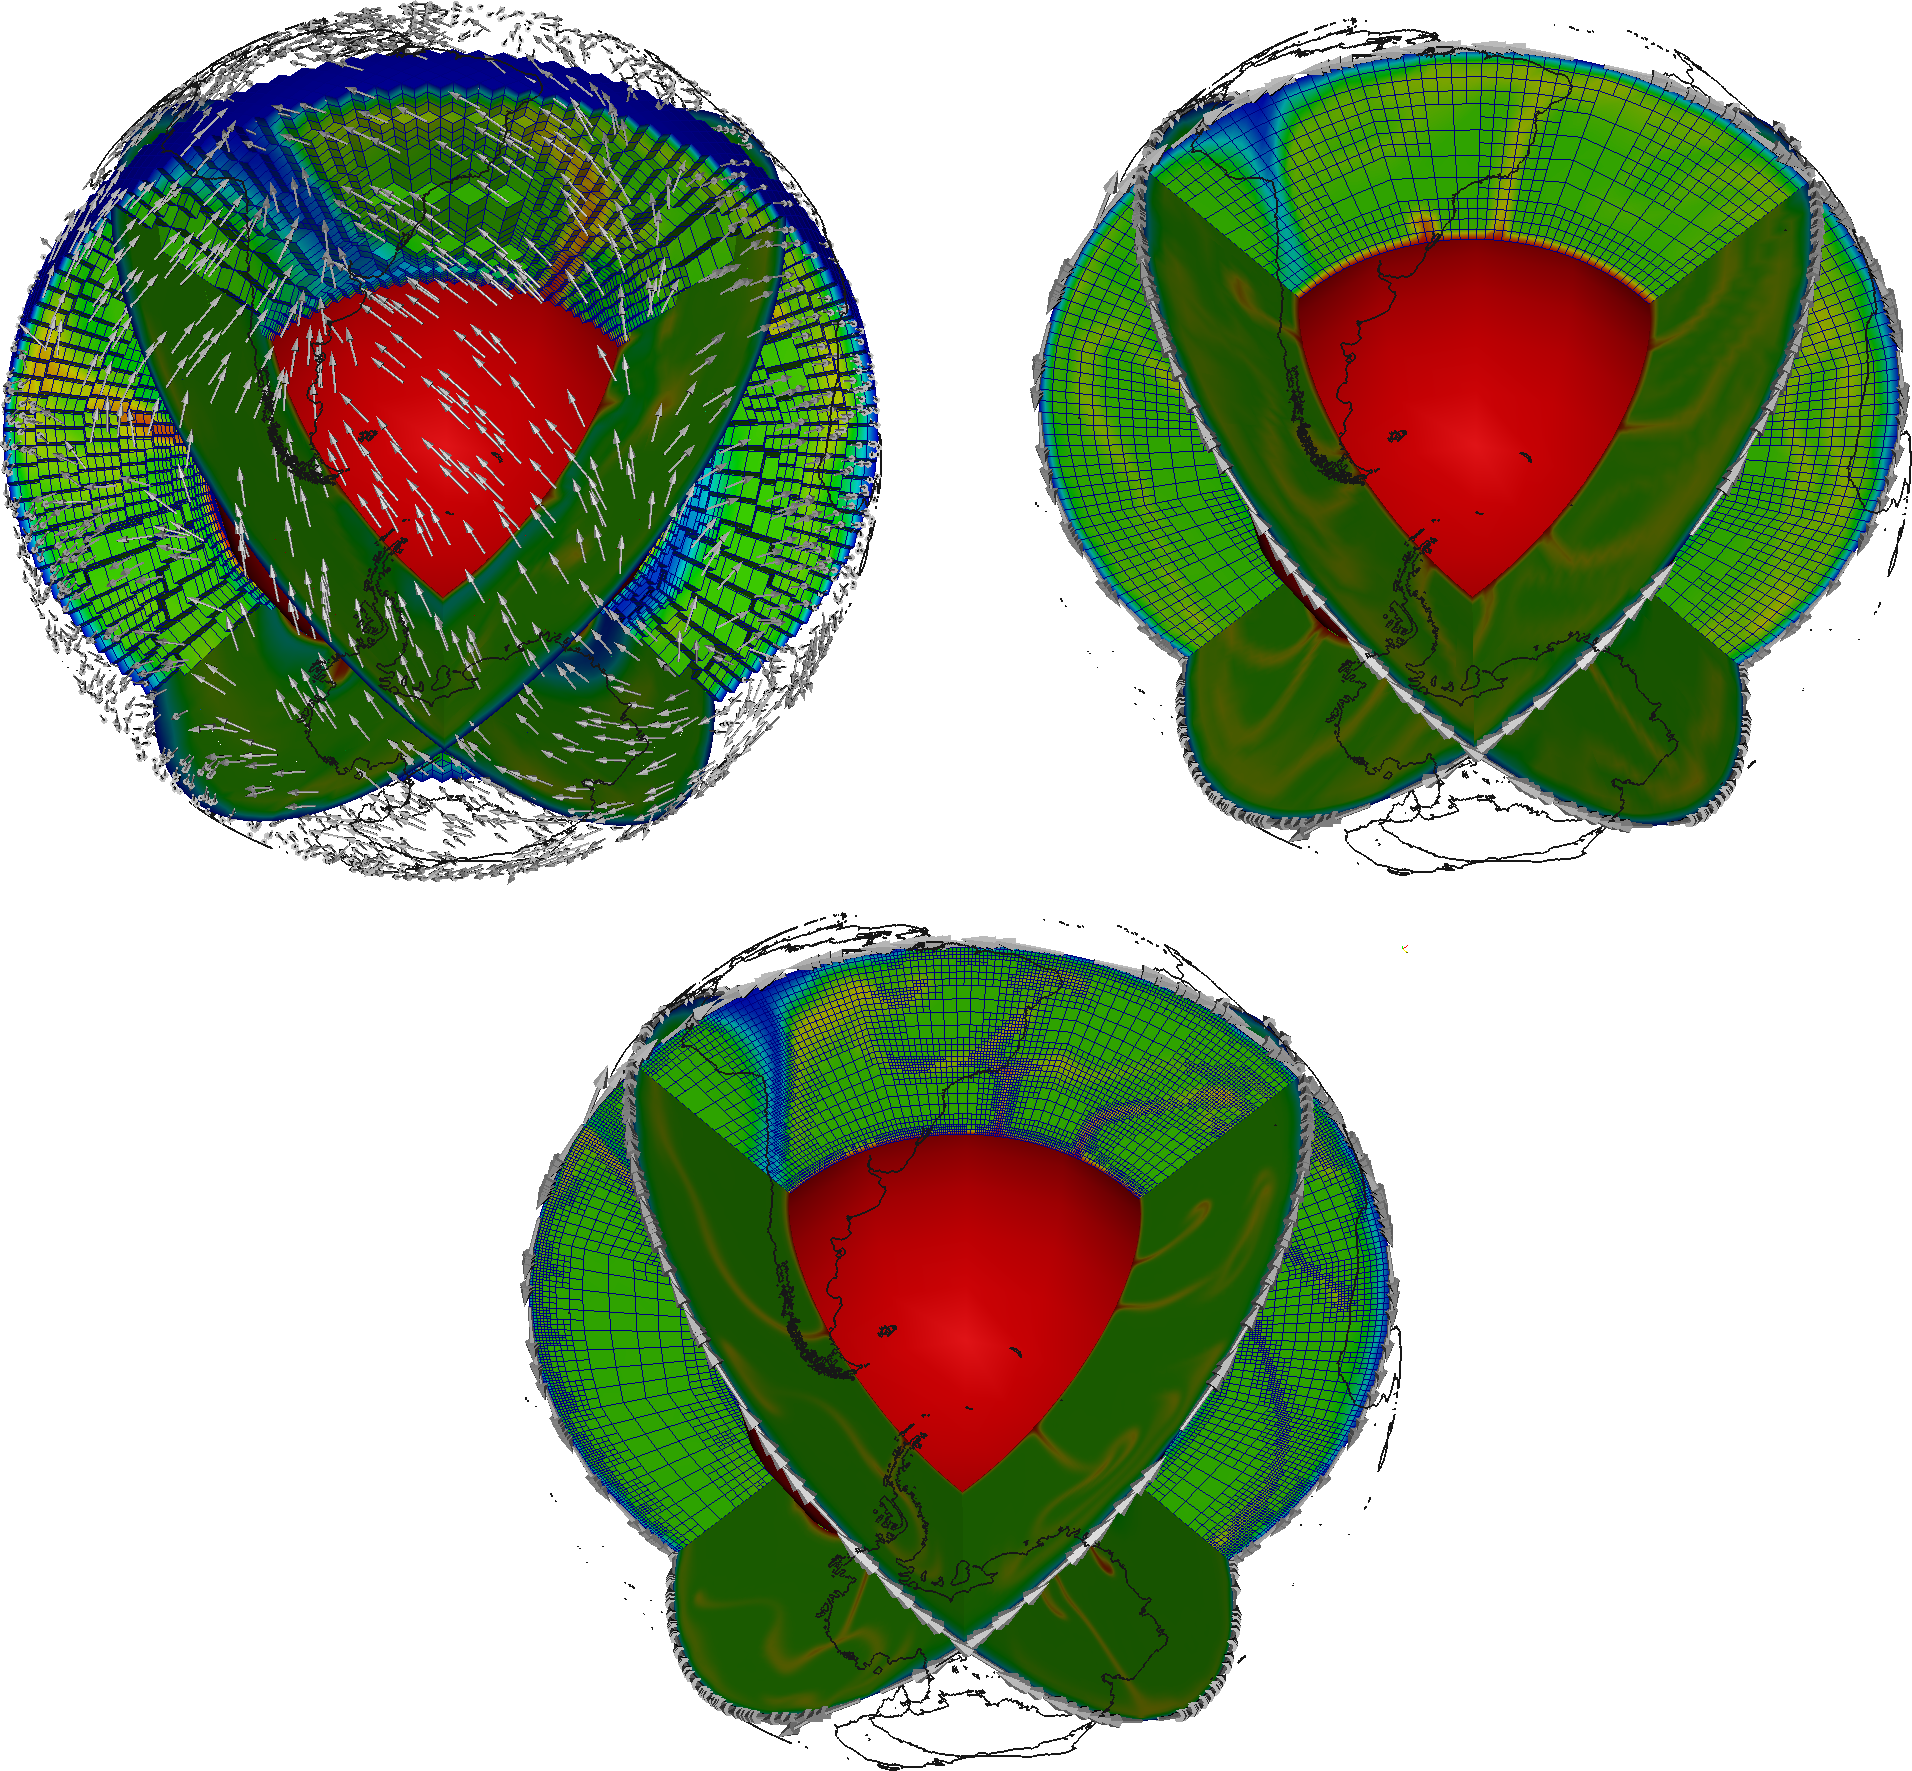
\includegraphics[width=\textwidth]{gplates-comparison.png}
  \hfill
  \caption{\it Using GPlates for velocity boundary conditions: The top left figure shows
  the results of a three-dimensional model using the present day plate velocities
  provided by GPlates as surface boundary condition. 
  The top right figure shows three independent computations 
  on two-dimensional slices through Earth. The boundary conditions for each of these slices (white
  arrows) are tangential to the slices and are projections of the
  three-dimensional velocity vectors into the two-dimensional plane
  occupied by the slice. While the two top models are created with the same mesh resolution
  the bottom figure shows three independent two-dimensional models using a higher resolution. 
  The view is centered on South America with Antarctica being near the bottom of
  the figure (coastlines provided by NGU and the GPlates project).}
  \label{fig:gv-1}
\end{figure}

\paragraph{Time-dependent boundary conditions.}
\label{sec:time-dependent-gplates-velocities}
The example presented above uses a constant velocity boundary field that
equals the present day plate movements. For a number of purposes one may want to
use a prescribed velocity boundary condition that changes over time, for example
to investigate the effect of trench migration on subduction. Therefore \aspect{}'s
GPlates plugin is able to read in multiple velocity files and linearly interpolate
between pairs of files to the current model time. To achieve this, one needs
to use the \texttt{\%d} wildcard in the velocity file name, which represents the current
velocity file index (e.g. \texttt{time\_dependent.\%d.gpml}). This index is
calculated by dividing the current model time by the user-defined time step
between velocity files (see parameter file above). As the model time progresses
the plugin will update the interpolation accordingly and if necessary read in
new velocity files. In case it can not read the next velocity file, it assumes
the last velocity file to be the constant boundary condition until the end of
the model run. One can test this behavior with the provided data files
\texttt{data/boundary-velocity/gplates/time\_dependent.\%d.gpml}
with the index \texttt{d} ranging from 0 to 3 and representing the plate movements of
the last 3 million years corresponding to the same plate reconstruction as used
above. Additionally, the parameter \texttt{Velocity file start time} allows for
a period of no-slip boundary conditions before starting the use of the GPlates plugin.
This is a comfort implementation, which could also be achieved by using the checkpointing
possibility described in section~\ref{sec:checkpoint-restart}. 
